%!TEX root = ../document.tex
\chapter{Empirical settings and methods}
In this chapter...

\section{Empirical setting}
The collection of data material used in this thesis took part in the late autumn, 2013, at a high school located in the center of Oslo. The school is in the upper third on the grade scale, with a limit of 43.5 points for admission in 2010/2011 \citep{utdanningsetaten}. Therefore the students at this school are mostly high achievers. 

Contact with the school was first initiated through Intermedia, and a presentational flier was sent as an explanation of the project (insert an appendix ref here). Luckily our request coincided perfectly with a two-week time frame for reviewing photosynthesis in one of the teacher's biology classes. He was therefore quite eager to swap out the experiment described in the textbook with an experiment using our application. 

The class selected for the experiment was a biology class at the highest level offered at the school, biology 2, which has an extensive curriculum covering e.g photosynthesis, enzymes and energy transmitters (insert ref to photosynthesis chapter). The students were between 17 and 18 years of age, and for the main part most of the 20 students taking the class were present. All the students agreed to participate in the study, but due to technical limitations and a busy time schedule, most of the data collection was only done with a small sample of the group. 

\subsection{Experiment}
\subsubsection{Planning}
The planning of the project was done by us in conjunction with the teacher responsible for the for the biology class. An initial planning meeting was held at the school around one week prior to the experiments. There we gave the teacher a thorough introduction of the system, and presented some ideas for expirements the students could conduct using our system as platform. This involved:

\begin{enumerate}
\item{Present the application in class}
\item{Initiate an experiment using the application. Related to e.g soil moisture, light intensity, light quality, or temperature}
\item{Have a one hour session where the students work with text tasks related to the experiment}
\end{enumerate}

The teacher then suggested that we could conduct two experiments, so the students could work on the relations between the different external factors effect on photosynthesis. As the system records a range of different variables, it would be possible to keep the environment relatively controlled, or at least point to factors which could be sources of error in the experiment. 

We agreed that the factor where we could get the most interesting result was to vary the light intensity and the light quality (wavelength). The first experiment would then involve keeping the plant located in a window facing west, receiving sunlight and light from the fluorescent indoor-lighting. In the second experiment we would plant new seeds, and relocate the plant to a (presumably) light proof cupboard. The plant would then only be given green light with a known wavelength. Each of the experiments would have a duration of approximately one week. 

\subsubsection{The experiments}
The project was presented and the first experiment initiated by one of the students on Friday 25th of October. This went on until Friday 1st of November when the second experiment was initiated. The second experiment went on until Wednesday 13th of November when the primary data collection session took place. During the experiments we were present at four separate occasions, observing what the teacher was focusing on, and which parts of the photosynthesis the students found most difficult. In addition we were answering questions about the system, and observed how the system was used by the teacher and how the students related to it. 

\subsubsection*{The plant in the window}
The first experiment was conducted with a setup in the window as shown in figure~\ref{fig:windowplant}. The system was located in the front of the classroom near a door leading to the next classroom, this meant it was visible and in reach of everyone walking by. The system was in the windowsill and there was a radiator located on the wall just beneath the plant. The plant was exposed to sunlight or daylight depending on the weather, but it was also exposed to the fluorescent indoor-lighting in the ceiling. Due to the time of year, and lack of people using the classroom in the evening, this meant that the plant would get light in the period between 08:00 and about 17:00. It turned out that the system was draining power from a power outlet that was either connected to the light, or timer based, since the system went down and did not post data between 19:00 and 07:00. We did also have some technical issues with the system the weekend from 25th of October to 27th of October, meaning that we missed data from the first seeds germinating.

\begin{figure}
\centering
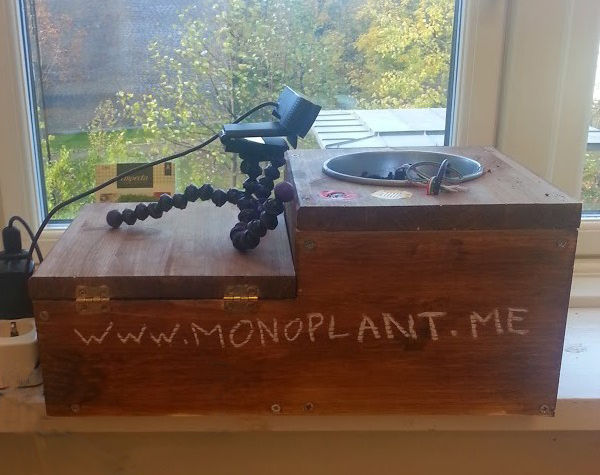
\includegraphics[width=0.8\textwidth]{img/empiricalsetting/window.jpg}
\caption{Image of the system located in the window}
\label{fig:windowplant}
\end{figure}



\subsubsection*{The plant in the cupboard}
The second experiment was conducted with a setup in a cupboard as shown in figure~\ref{fig:cupboardplant}. The cupboard was located in the front of the classroom, however more stuck in the corner behind the teachers desk. However, this picture is taken with flash and light from the room coming in to the cupboard.

\begin{figure}
\centering
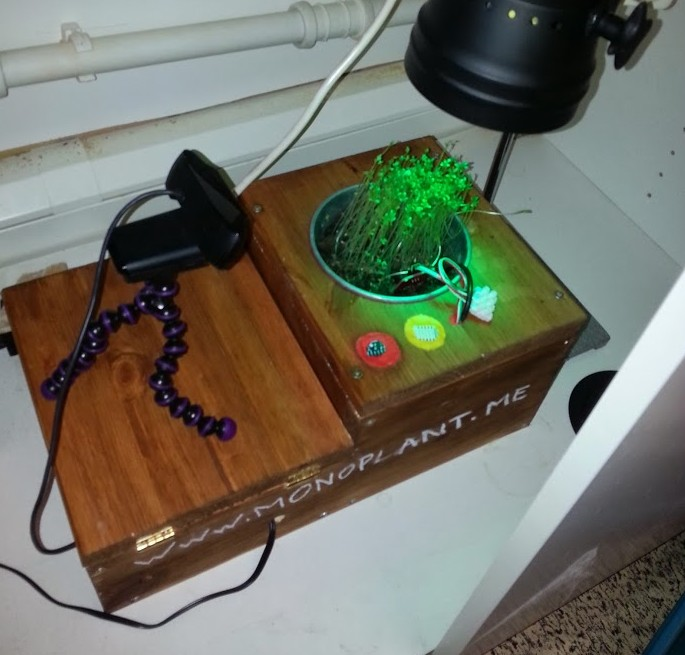
\includegraphics[width=0.8\textwidth]{img/empiricalsetting/cupboard.jpg}
\caption{Image of the system located in the cupboard}
\label{fig:cupboardplant}
\end{figure}


\subsection{Data collection}
Different methods for data collection was discussed and reviewed early on in the project. As our primary data source we chose video data with the use of multiple cameras and a screen-dump. This was collected only during one session lasting 45 minutes, resulting in 3x45 minutes of video data and 1x45 minutes of audio data. Supplementary data from this session includes the written answers from the groups which were not filmed, and our personal notes of general observations. In addition to this we were present at five occasions preceding the session, taking notes. In the following sections the methods used will be discussed. 

\subsubsection{Video and audio}
It was determined early in the project that video and audio recording were to be used. Perhaps the primary reason for this was the tradition at Intermedia, as video data collection has been used and thoroughly tested by a number of researchers here. This meant that we would get a lot of help from co-located researchers in what microphones to use, placement of cameras, operation of the equipment, etc. 

A total of 45 minutes of video and audio was recorded, using three separate video sources, and three microphones. One camera was placed in front of the group, able to capture facial expressions
\begin{figure}
\centering
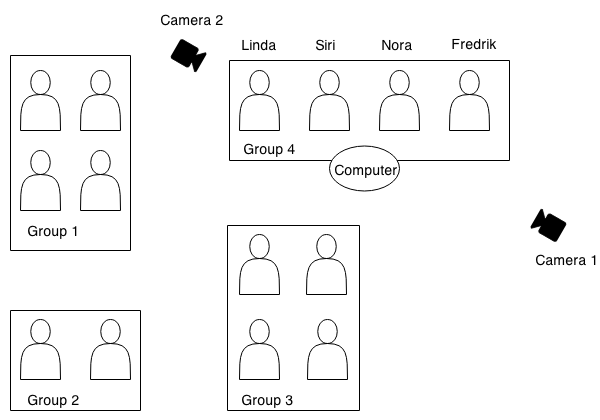
\includegraphics[width=0.8\textwidth]{img/empiricalsetting/class_diagram.png}
\caption{Camera setup}
\label{fig:camerasetup}
\end{figure}

The main advantage with using video is the ability to replay a sequence as many times as necessary. This gives us the ability to give thick descriptions of what happened without being compromised by the human memory capacity.

\subsubsection{Passive observation}

\subsubsection{Document analysis}

\subsubsection{Web logs}

Our most influential source, regarding both paradigm, methodology and method were the tradition for using qualitative data in information systems research at department of informatics. 



\subsection{Analytical Procedures}
\subsubsection{Interaction analysis}
%Crang & cook: Video recordings can be criticized by pointing out that it is the researcher that selects the frame and focus. Hence the data can become biased. However, by trying to frame interaction generically, and providing a video, getting other people to double check coding and transcription.
The analytical procedure employed within this thesis is \emph{Interaction analysis} \citep{jordan1995interaction}, an interdisciplinary method which emerged from fields such as ethnography, sociolinguistics, ethnomethodology, conversation analysis, and sociocultural theories. 

\begin{quote}
An interdisciplinary method for the empirical investigation of the interaction of human
beings with each other and with objects in their environment. It investigates human
activities such as talk, nonverbal interaction, and the use of artifacts and technologies,
identifying routine practices and problems and the resources for their solution \citep[p39]{jordan1995interaction}
\end{quote}

For Interaction analysis to become a reality video and audio recording technology has been a vital resource. The combination of recording talk as well as nonverbal interaction and the ability to replay a sequence as many times as necessary gives us the possibility to analyze more thoroughly. Combining this micro-level data of interaction with ethnographic data gives us a means of analyzing how the interaction is part of the situated context and institutional practices. \citep{furberg2009scientific}. 

Even though we have done a case study in a real educational setting, considering these ethnographic data is important if we are to keep a dialogic perspective. 

How we 


\subsubsection{Making sense of the data}
\citeauthor{derry2010conducting} speaks about two different approaches to select parts of a video corpus for further examination. These two are the \emph{inductive} approach and the \emph{deductive} approach, where we clearly fit into the inductive apporach.

To make sense of the data gathered we approached it in several different ways with different focuses. Below is a chronological list of the ways we approached the data. 

\begin{enumerate}
\item{Viewing recordings locating interesting interaction}
\item{Divide recordings between us for audio transcription}
\item{Watching screen-cast to make additional notes on interaction with the system}
\item{Watching the recordings with our supervisor and discuss what we think is important}
\end{enumerate}

\subsection{Ethics}



